\hypertarget{ux8d21ux732eux8005ux4f4dux7f6e}{%
\subsubsection{贡献者位置}\label{ux8d21ux732eux8005ux4f4dux7f6e}}

问题:贡献者的位置在哪里?

\hypertarget{ux63cfux8ff0}{%
\paragraph{描述}\label{ux63cfux8ff0}}

贡献者所处的地理位置、居住地或工作地。

\hypertarget{ux76eeux6807}{%
\paragraph{目标}\label{ux76eeux6807}}

用于确定贡献者的全球位置,了解他们的工作实践和时区。
确定没有贡献的区域,以提高这些区域的参与度;

\hypertarget{ux5b9eux73b0}{%
\paragraph{实现}\label{ux5b9eux73b0}}

\hypertarget{ux7b5bux9009ux6761ux4ef6}{%
\subparagraph{筛选条件}\label{ux7b5bux9009ux6761ux4ef6}}

按以下条件筛选贡献:

\begin{itemize}
\tightlist
\item
  **位置。**将各区域的位置分组,以进行多级报告。
  在此语境中,``位置''是一个故意模糊的术语,可以指地区、国家、州、地域或时区。
\item
  **时间段。**开始日期和完成日期。 默认:永久。 计算贡献的时期段。
\item
  \textbf{贡献者类型},例如:

  \begin{itemize}
  \tightlist
  \item
    仓库作者
  \item
    议题作者
  \item
    代码审查(Code Review)参与者
  \item
    邮件列表作者
  \item
    事件参与者
  \item
    IRC 作者
  \item
    博客作者
  \item
    按发布周期
  \item
    项目的编程语言
  \item
    项目中的角色或职能
  \end{itemize}
\end{itemize}

\hypertarget{ux53efux89c6ux5316ux6548ux679c}{%
\subparagraph{可视化效果}\label{ux53efux89c6ux5316ux6548ux679c}}

点密度图:

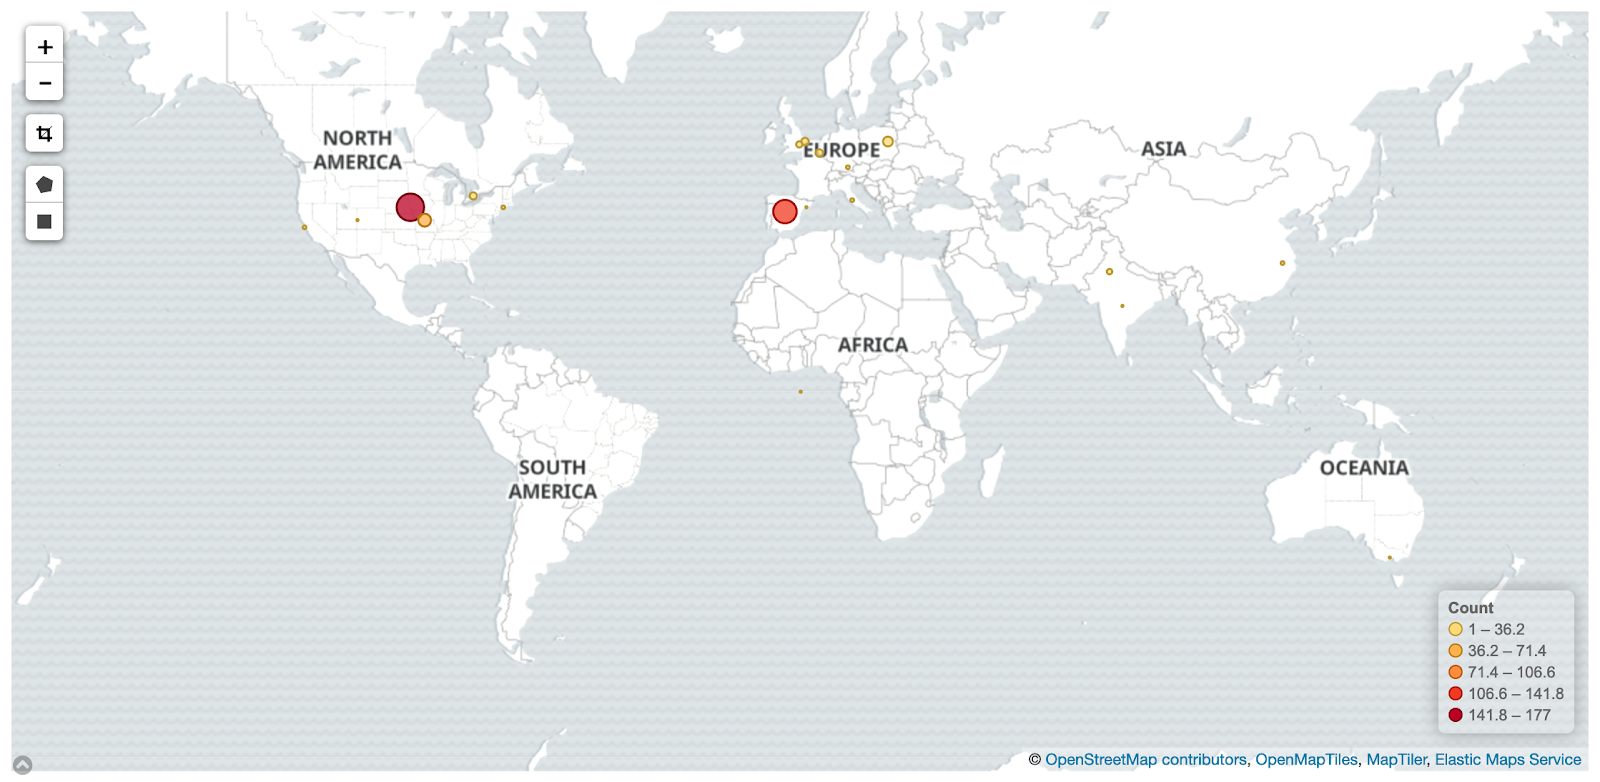
\includegraphics{images/contributor-location_dot-density-map.png}

来源:\href{https://chaoss.biterg.io/goto/a62f3584a41c1c4c1af5d04b9809a860}{https://chaoss.biterg.io/goto/a62f3584a41c1c4c1af5d04b9809a860}

可视热图:

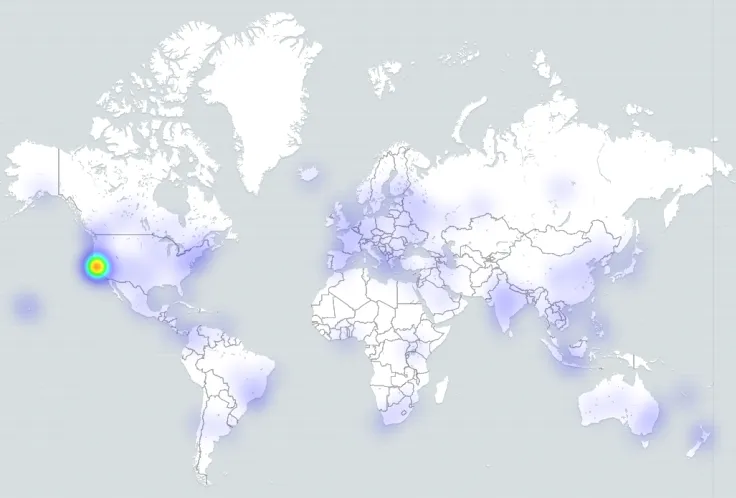
\includegraphics{images/contributor-location_heatmap.png}

来源:
\href{https://blog.bitergia.com/2018/11/20/ubers-community-software-development-analytics-for-open-source-offices}{https://blog.bitergia.com/2018/11/20/ubers-community-software-development-analytics-for-open-source-offices}

\hypertarget{ux63d0ux4f9bux5ea6ux91cfux7684ux5de5ux5177}{%
\subparagraph{提供度量的工具}\label{ux63d0ux4f9bux5ea6ux91cfux7684ux5de5ux5177}}

\begin{itemize}
\tightlist
\item
  GrimoireLab
\item
  Augur
\end{itemize}

\hypertarget{ux6570ux636eux6536ux96c6ux7b56ux7565}{%
\subparagraph{数据收集策略}\label{ux6570ux636eux6536ux96c6ux7b56ux7565}}

可以采用不同的方法收集位置信息:

\begin{itemize}
\tightlist
\item
  在参与度系统中收集贡献者资料的位置信息。
\item
  使用做出贡献的最频繁位置的 IP 地址地理定位。
\item
  根据贡献中的时间戳推断地理位置。
\item
  调查贡献者。
\end{itemize}

确定贡献者的位置是数据收集的关键挑战。
最佳实践是利用参与度系统提供的各种资料信息,如果没有这些信息,可以使用
IP 地理定位来确定该个人最频繁的贡献位置。
注意,贡献者可能会在个人资料信息中输入虚假或无意义的位置信息(如``地球''或``互联网'')。
注意,IP 地理定位可能会由于 VPN 或其他 IP 屏蔽工具提供大量误报。

另一个考虑因素是外部数据收集工具,如社区调查或事件登记数据,可能交叉引用参与概况的系统。
贡献者位置数据可与事件\href{https://chaoss.community/metric-attendee-demographics/}{参与者统计信息}和\href{https://chaoss.community/metric-speaker-demographics/}{演讲者统计信息}内联收集。

\hypertarget{ux53c2ux8003ux8d44ux6599}{%
\paragraph{参考资料}\label{ux53c2ux8003ux8d44ux6599}}

\begin{itemize}
\tightlist
\item
  Gonzalez-Barahona, J. M., Robles, G., Andradas-Izquierdo, R., \&
  Ghosh, R. A. (2008). Geographic origin of libre software developers.
  \emph{Information Economics and Policy}, \emph{20}(4), 356-363.
\end{itemize}
